In \autoref{abb:ProdukteDB} werden verwendbare Dienste für die Batch (\enquote{\ac{OLAP}}) Verarbeitung von \ac{AWS}, gemeinsam mit ihren jeweiligen Einsatzgebieten gezeigt. In diesem Abschnitt soll besonders auf die Dienste zur Verarbeitung nach dem Laden der Daten in eine der gezeigten Datenquellen eingegangen werden. Gezeigt werden jedoch auch Dienste für Datenvisualisierung und Machine Learning, da diese komplementär oder mit den prozessierten Daten verwendet werden können. Da die einzelnen Datenquellen jeweils verschiedene Sprachen, bzw. Dialekte von \ac{SQL} verwenden, sind die spezifischen Abfragesprachen mit einem generischen Eintrag in der Grafik abgebildet. Dabei ist es bei \ac{AWS} durchaus üblich, Interoperabilität zu anderen \ac{AWS} Diensten, wie beispielsweise Lambda, in den jeweiligen \ac{SQL} Dialekt einzubauen.

\begin{figure}[H]
\centering
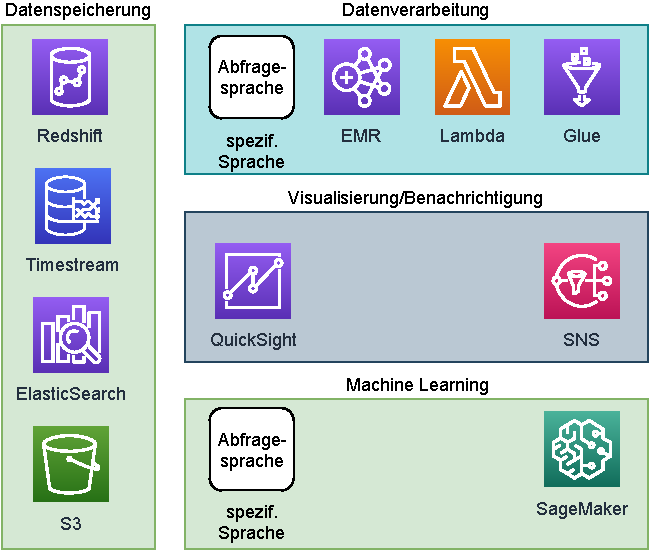
\includegraphics[width=\textwidth]{graphics/Overview-DB.pdf}
\caption{Einsetzbare Produkte im Bereich Datenbankverarbeitung}
\label{abb:ProdukteDB}
\end{figure}


\subsection{Amazon Timestream}
Timestream ist nach Aussage des Herstellers eine schneller, skalierbare und speziell für Zeitreihendaten entwickelte Datenbank, welche über \ac{AWS} als Dienstleistung bezogen werden kann.\footcite[Vgl. auch im Folgenden][]{AmazonWebServicesInc..o.J.h} Timestream integriert zwei verschiedene Speichertypen, nämlich \ac{RAM}-basierten Speicher, in dem Daten, auf welche schnell zugegriffen werden sollen, gespeichert werden können und Festplatten-basierten Speicher, welcher für historische Daten dienen soll.
Timestream besitzt zusätzlich einen eigenen \ac{SQL}-Dialekt, welcher um Funktionen zur Analyse von Zeitreihendaten erweitert wurde. Ein Beispiel für den Einsatz des \ac{SQL}-Dialekts zur Abfrage der Informationen für den Anwendungsfall, der zum Kostenvergleich beschrieben wurde, ist in \autoref{listing:timestream-kostenvergleich} zu sehen.

\begin{listing}[H]
\inputminted[frame=lines,breaklines=true]{sql}{code/timestream-threshold.sql}
\caption{Abfrage für Kostenvergleichs Usecase}
\label{listing:timestream-kostenvergleich}
\end{listing}

Timestream ist nicht selbst in der Lage, Abfragen zu planen. \ac{AWS} gibt in der Dokumentation selbst an, dass Lambda verwendet werden kann, um periodisch eine Abfrage in Timestream auszuführen und basierend auf dieser Anfrage Alarme via \ac{SNS} zu versenden.\footcite[Vgl.][]{AmazonWebServicesInc..o.J.ag} Abgebildet ist diese Interaktion in \autoref{abb:TimestreamLAmbdaOrchestration}.


\begin{figure}[H]
\centering
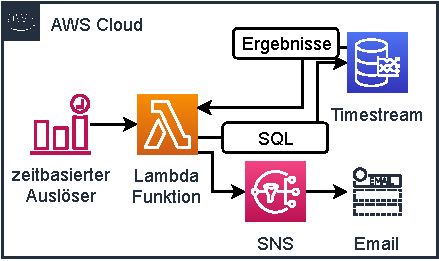
\includegraphics[width=0.45\textwidth]{graphics/Lambda-Timestream-Orchestration.pdf}
\caption{Orchestrierung von zeitbasierten Timestream Abfragen}
\label{abb:TimestreamLAmbdaOrchestration}
\end{figure}

\subsubsection{Featurevergleich}
Perzentile lassen sich mit der eingebauten Funktion \mintinline{sql}{approx_percentile(x, percentage)} berechnen, der Mittelwert via \mintinline{sql}{avg(x)} oder \mintinline{sql}{geometric_mean(x)}

Eine native Anomalieerkennung bietet Timestream nicht, jedoch kann die Machine Learning Dienstleistung Amazon SageMaker Daten von Timestream analysieren und Anomlieerkennung ausführen.\footcite[Vgl. auch im Folgenden][]{AmazonWebServicesInc..o.J.aj} In SageMaker kann auch der nativ in Kinesis Data Analytics verbaute Random Cut Forest Algorithmus verwendet werden, um Anomalien zu erkennen. Andernfalls kann, wie von \citeauthor{Salgado.2019} beschrieben, eine einfache Anomalieerkennung durch Überprüfung des Wertes auf Lage ziwschen 25. und 75. Quantil erfolgen.\footcite[Vgl.][]{Salgado.2019}

Die Schwellwertüberschreitungserkennung ist mittels einer einfachen \mintinline{sql}{WHERE} Bedingung machbar.

Ein gleitender Durchschnitt ist, wie von \citeauthor{Ross.2020} gezeigt, in SQL mittels der Bearbeitungsfenster, die Timestream, wie viele andere \ac{SQL} Implementierungen anbietet, möglich.\footcite[Vgl.][]{Ross.2020} Gleichzeitig unterstützt Amazon Timestream die Verwendung von Ableitungen als Werkzeug zur Trenderkennung.\footcite[Vgl.][]{AmazonWebServicesInc..o.J.ai}

\subsubsection{Performancevergleich}
Die \ac{SLA} von Timestream bietet allein 99,99\% Verfügbarkeit pro Verrechnungsmonat.\footcite[Vgl.][]{AmazonWebServicesInc..2020d} \ac{AWS} verspricht aber eine bis zu tausendfache Geschwindigkeitsverbesserung gegenüber relationalen Datenbanken.\footcite[Vgl.][]{AmazonWebServicesInc..o.J.ak}

Mitbewerber von \ac{AWS} im Bereich der Zeitseriendatenbanken haben in ihren Tests festegestellt, dass Timestream langsamer als ihre Konkurrenzprodukte waren.\footcite[Vgl.][]{Booz.2020}\nzitat\footcite[Vgl.][]{Crate.ioInc..2020} Dabei sind die Testskripte von \citeauthor{Booz.2020} Open Source und damit die Messungen theoretisch reproduzierbar. Gleichzeitig gibt \ac{AWS} aber in einem Blogeintrag aus dem November an, Datensätze im Bereich von einem bis 21,7 TB analysieren zu können, ohne 100 Sekunden Ausführungszeit zu überschreiten.\footcite[Vgl.][]{Das.2020} Auch für diese Tests ist der Quellcode open source verfügbar.

Es kann also keine finale Aussage über die genauen Performancegarantien getroffen werden, da entweder den Mitbewerbern von \ac{AWS} Glauben zu schenken ist, oder \ac{AWS} selber. Da es im kommerziellen Interesse aller Parteien liegt Timestream entweder auf- oder abzuwerten ist eine stichhaltige Aussage also nicht möglich.

\subsubsection{Kostenvergleich}


Timestream ist momentan noch nicht in Frankfurt verfügbar, weshalb die Kosten in der einzigen europäischen Zone mit verfügbarem Timestream, Irland, als Maßstab verwendet werden. Angenommen wird, dass die Daten eine Stunde im \ac{RAM} vorgehalten werden und danach in die Festplattenspeicherung überführt werden.

%  Angenommen 8.640.000 (8,64 GB)/Monat 0,012GB/h 4,885056
% Abfrage: 25,92 GB

Ausgehend von dem beschriebenen Szenario lässt sich nicht genau errechnen, welche Datenmenge von den Anfragen genau erfasst wird. Dies ist dem Fakt geschuldet, dass Timestream die Daten optimiert abspeichert und nur den tatsächlichen Messwert speichert. Numerische Daten können als 32-bit int, als 64bit BigInt oder als 64bit double gespeichert werden.\footcite[Vgl. auch im Folgenden][]{AmazonWebServicesInc..o.J.r}\nzitat\footcite[Vgl. auch im Folgenden][]{AmazonWebServicesInc..o.J.q} Wenn dazu ein String für die Sensorid im Stile \enquote{Sensor-123} angenommen wird, der 19 bytes zur Darstellung benötigt und der Zeitstempel addiert wird, der 8 bytes benötigt, ergibt sich eine Speicherbelegung von 91 Bytes. Speicherkosten werden aber bei Werten unter einem Kilobyte auf einen Kilobyte hochgerundet, weshalb dies in der Speicherrechnung keine Beachtung findet. Wenn man weitere Optimierungen, die die Abfrageengine macht außer Acht lässt, muss mit 0,78624GB pro abgefragtem Monat gerechnet werden.

\Todo{Lambda Orchestration hinzufügen}
\begin{table}[H]
\centering
\begin{tabular}{|l|l|l|}
\hline
Dimension & Preis(\$)/Einheit & Summe (\$) \\ \hline
Schreibzugriffe & 0,5654/Mio./KB & 4,885056 \\ \hline
\begin{tabular}[c]{@{}l@{}}\ac{RAM} \\ Speicherung\end{tabular} & 0,0407/GB/h & 0,351648 \\ \hline
\begin{tabular}[c]{@{}l@{}}Festplatten\\ Speicherung\end{tabular} & 0,0339/GB/Monat & 0,878688 \\ \hline
Anfragen & \begin{tabular}[c]{@{}l@{}}0,011308/GB \\ abgefragt\end{tabular} & 25,6055095296 \\ \hline
Summe & \cellcolor[HTML]{EFEFEF} & 31,7209015296 \\ \hline
\end{tabular}
\caption{Kostenvergleich AWS~Timestream}
\label{tab:kostenvergleich-AWS~Timestream}
\end{table}

% \subsubsection{Gesamtbewertung}
% \produktbewertung{Amazon~Timestream}{x,10,7,8,7,5,3,4,2,1,0,x}

\subsection{Amazon Athena}\label{chap:athena}


Amazon Athena ist nach Aussage des Herstellers ein voll verwalteter Query Dienst, welcher das Durchsuchen von großen Datenmengen im \ac{S3} Speicherdienst möglich macht.\footcite[Vgl.][]{Barr.2016} Athena basiert dabei auf dem ursprünglich von Facebook entwickelten Presto, welches mittlerweile Open Source ist. Innerhalb von Athena können Daten verschiedener Formate (\ac{CSV}, Apache Parquet, Apache ORC, \ac{JSON}, ...) mittels \ac{SQL} verarbeitet werden. Zusätzlich ist seit November 2020 mittels der sogenannten \enquote{Federated Queries} auch die Abfrage von anderen Datenquellen wie Apache HBase, Amazon Document DB oder von Datenquellen, die durch eigenentwickelte Verbindungselemente verknüpft werden.\footcite[Vgl.][]{AmazonWebServicesInc..o.J.s} Technisch werden diese Federated Queries via Lambda abgewickelt.

Bei verändernden Datenschemata wird empfohlen, den Dienst \ac{AWS} Glue Crawler komplementär einzusetzen, welcher die Schemata aus \ac{S3} automatisch extrahiert und in Athena hinterlegt. Andernfalls können die Schemata auch manuell hinterlegt werden.

\subsubsection{Featurevergleich}
Die technische Grundlage für Athena, Presto bietet mit \mintinline{sql}{approx_percentile(x, percentage)} eine Funktion zur Kalkulation von Perzentilen an.\footcite[Vgl.][]{ThePrestoFoundation.o.J.}

Eine Möglichkeit, um Anomalien in Athena zu erkennen, ist es alle Werte, die ausserhalb der Spanne zwischen dem 25. und 75. Quantil liegen als Anomalie zu klassifizieren.\footcite[Vgl.][]{Salgado.2019} Dies wäre mit der \mintinline{sql}{approx_percentile(x, percentage)} Funktion von Athena machbar. Andernfalls könnte wie von \citeauthor{Megler.2016} vorgeschlagen, der Amazon \ac{EMR} Dienst benutzt werden, um Anomalien mittels der Bildung von Clustern und der Kalkulation der Distanz von Werten zu diesen Clustern zu detektieren.\footcite[Vgl.][]{Megler.2016}

Schwellwertüberschreitungen können via einer \mintinline{sql}{WHERE} Bedingung, wie bei Timestream auch, erkannt werden.

Wie bei Timestream auch kann nach der Methode von \citeauthor{Ross.2020} ein gleitender Durchschnitt mittels der Verarbeitungsfenster kalkuliert werden.\footcite[Vgl.][]{Ross.2020}

\subsubsection{Performancevergleich}

\citeauthor{Hartland.2018} beschreiben einen Anwendungsfall, in dem sie Athena zur Analyse von Logdaten innerhalb der Datenanalyseinfrastruktur des ATLAS Experiments am Large Hadron Collider im CERN Forschungszentrum bei Genf verwenden.\footcite[Vgl.][]{Hartland.2018}

Gleichzeitig stellen \citeauthor{Hartland.2018} auch fest, dass es Teil des Entwicklungsprozesses ist, die Anfragen zu  optimieren, um Kosten zu sparen.\footcite[Vgl.][5]{Hartland.2018} Dies entstammt der Natur von \ac{SQL} basierten Abfragemechanismen, da verschiedene Abfragestile und Operationen auf verschieden viele Speicherpartitionen zugreifen müssen. Da Athena nach Volumen der Speicherzugriffe abrechnet, kann es also sinnvoll sein, den Speicher nach Abfragearten zu partitionieren oder die Abfragen zu optimieren. Dazu können der im April 2021 vorgestellten \mintinline{sql}{EXPLAIN} \ac{SQL}-Befehl und die damit zusammenhängenden query execution plans verwendet werden.\footcite[Vgl. auch im Folgenden][]{AmazonWebServicesInc..2021} Diese zeigen nach Aussage von \ac{AWS} auf, wie eine Abfrage ausgeführt werden würde und wie Laufzeiten optimiert werden können.

Die reale Performance der bearbeiteten Anfragen garantiert \ac{AWS} nicht. Da Athena ein serverless Dienst ist, dessen unterleigende Kapazität vollständig von \ac{AWS} verwaltet wird, können Nutzende keinen Einfluss auf die provisionierten Ressourcen nehmen. Zusätzlich hängt die Performance stark von der Partitionierung der Daten und der Kompression ab.\footcite[Vgl.][]{Levy.2021} Zusätzlich zu beachten ist, dass Athena eine Limitierung von 20 (25 in der North Virginia Region) parallel laufenden/wartenden Anfragen hat und Anfragen nach 30 Minuten Laufzeit abgebrochen werden. \footcite[Vgl. auch im Folgenden][]{AmazonWebServicesInc..o.J.ac} Diese Limitierungen können jedoch auf Anfrage erhöht werden.

Amazon garantiert vertraglich keine Performance, sondern nur die 99,99\% Verfügbarkeit des Dienstes in dem \ac{SLA}.\footcite[Vgl.][]{AmazonWebServicesInc..2019c} In Vergleichen von \citeauthor{Levy.2019} und \citeauthor{Khadtare.2018} mit dem Mitbewerber Google BigQuery zeigte Athena schlechtere Performance, gemessen an den Antwortzeiten der Abfragen, war aber günstiger.\footcite[Vgl.][]{Levy.2019}\nzitat\footcite[Vgl.][]{Khadtare.2018} Da \ac{AWS} Ende 2020 mit Athena engine version 2 wesentliche Performanceverbesserungen angekündigt hat, ist außerdem fraglich, ob die Daten noch aktuell sind.\footcite[Vgl.][]{AmazonWebServicesInc..2020c}

\subsubsection{Kostenvergleich}
Für die Folgende Kostenbewertung wird angenommen, dass Athena die Daten aus \ac{S3} indiziert, welche im \ac{JSON} Format gespeichert werden. Zu beachten ist, dass effizientere Formate wie CSV, oder sogar Apache Parquet und ORC, welche komprimiert Daten speichern können, verwendet werden  könnten. Verwendung von Parquet oder ORC würde laut \ac{AWS} 30-90\% Kosten sparen.\footcite[Vgl.][]{AmazonWebServicesInc..o.J.t} Gleichzeitig kann aber eine Speicherung im \ac{JSON} Format via \AWSIOT{} Rule erfolgen, ohne dass weitere Verarbeitung notwendig ist.


\begin{figure}[H]
\centering
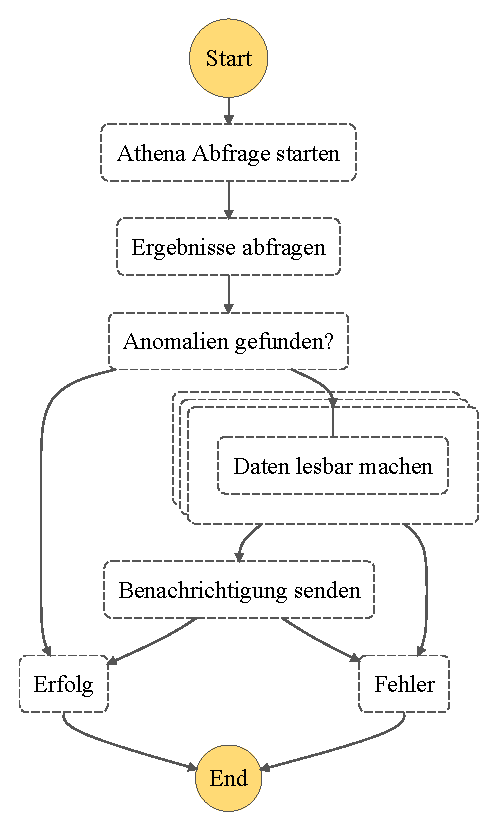
\includegraphics[height=0.45\textheight]{graphics/Step-Function-Athena.pdf}
\caption{Beispiel Step Function State Machine}
\label{abb:StepFunctionExample}
\end{figure}

In \autoref{tab:kostenvergleich-Amazon~Athena} wird davon ausgegangen, dass 2MB an Daten im Zeitraum von 10 Minuten neu hinzukommen. Da aber eine Historie gebildet werden soll, müssen sowieso die gesamten dreimonatigen historischen Daten abgefragt werden. Ausgehend von 200 kB pro Minute von allen Geräten ergeben sich 25,92 GB Datenvolumen an historischen Daten, welche 960 mal im Monat abgefragt werden sollen. Athena rundet dabei auf das nächste MegaByte auf und hat ein Minimum von 10 MB erfasster Daten pro Anfrage.\footcite[Vgl.][]{AmazonWebServicesInc..o.J.t} Das Datenschema für Athena stellt Glue bereit, welches Kosten für Abfragen aus dem Datenkatalog und Speicherkosten für den Datenkatalog erhebt.\footcite[Vgl.][]{AmazonWebServicesInc..o.J.u} Zur Orchestrierung wird ein Ablauf, wie in \autoref{abb:StepFunctionExample} gezeigt in StepFunctions abgebildet, welches für jeden Zustandsübergang eine Gebühr erhebt.\footcite[Vgl.][]{AmazonWebServicesInc..o.J.v}

\begin{table}[H]
\centering
\begin{tabular}{|l|l|l|}
\hline
Dimension & Preis(\$)/Einheit & Summe (\$) \\ \hline
Athena Abfragen & \begin{tabular}[c]{@{}l@{}}0,005/TB \\ abgefragte Daten\end{tabular} &  121,50\\ \hline
\begin{tabular}[c]{@{}l@{}}Glue Data Catalog\\ Speicher\end{tabular} & 1/100.000 Objekte &  \textless 0,0001\\ \hline
\begin{tabular}[c]{@{}l@{}}Glue Data Catalog\\ Abfragen\end{tabular} & 1/Million Abfragen &  \textless 0,0001\\ \hline
Step Functions & \begin{tabular}[c]{@{}l@{}}0,025/1000 \\ Zustandsübergänge\end{tabular} &  1,08\\ \hline
\ac{SNS} (Push) & \begin{tabular}[c]{@{}l@{}}0,00002/Nachricht\\ (angenommen 5 Alarme/Gerät/Monat)\end{tabular} & 0,02 \\ \hline
Summe & \cellcolor[HTML]{EFEFEF} &  122,60\\ \hline
\end{tabular}
\caption{Kostenvergleich Amazon~Athena}
\label{tab:kostenvergleich-Amazon~Athena}
\end{table}


% \subsubsection{Gesamtbewertung}
% \produktbewertung{Amazon~Athena}{x,x,x,x,x,x,x,x,x,x,x,x}


\subsection{Amazon Redshift}

Amazon Redshift ist der Data Warehouse Dienst von \ac{AWS}, welcher nach Aussage des Herstellers \enquote{enterprise-level} ist und auf ein Datenvolument von Petabytes skalieren kann. \footcite[Vgl.][1]{AmazonWebServicesInc..o.J.g} Redshift ist dabei ein klassisches \ac{OLAP} Produkt, welches für eine Vielzahl verschiedener Daten effizient Auswertungen bereitstellen kann. Redshift basiert auf der bekannten Open Source Datenbank PostgreSQL, weicht jedoch in der Implementierung diverser Kommandos und Features ab, die das Amazon als irrelevant für \ac{OLAP} Anwendungen hält.\footcite[Vgl.][4]{AmazonWebServicesInc..o.J.g}\nzitat\footcite[Vgl.][428\psqq]{AmazonWebServicesInc..o.J.g} Kern von Redshift sind sogenannte Cluster, welche aus einer oder mehrerer Berechnungsknoten (\enquote{compute nodes}) und Anführerknoten(\enquote{leader nodes}) besteht. Applikationen interagieren allein mit den Anführerknoten, die existierenden Berechnungsknoten sind zwar transparent für die Anwendung, werden jedoch von den Anführerknoten mit Ausführungsplänen versorgt, die diese entwickelt um Anfragen effizient zu verarbeiten.\footcite[Vgl.][4]{AmazonWebServicesInc..o.J.g}

Redshift bietet zusätzlich mit Redshift Spectrum einen Dienst an, welcher auf den ersten Blick dem in \autoref{chap:athena} vorgestellten Athena gleicht. Beide rufen via \ac{SQL} Daten von \ac{S3} ab und beide kosten 5\$/TB gescannte Daten.\footcite[Vgl. auch im Folgenden][]{Smallcombe.2020} Wichtige Unterschiede liegen dabei aber in der Art, wie Ressourcen verwaltet und genutzt werden können. Während Redshifft Spectrum nur in Kombination mit einem Redshift Cluster verwendet werden kann, funktioniert Athena ohne Kopplung an verwaltende Ressourcen. Gleichzeitig ist ein stärkerer Einfluss auf die Performance bei Redshift möglich, da man zusätzliche Clusterressourcen einfach provisionieren kann, während Athena vollständig von \ac{AWS} verwaltet wird. Entsprechend erlaubt Redshift Spectrum zwar größeren Einfluss auf die Performance von Datenabfragen, dieser Einfluss muss jedoch in Form von zusätzlich abzurechnenden Clusterressourcen abgerechnet werden, was Redshift für Anwendungsfälle, die keine gesichert gleichbleibende Performance benötigen, unattraktiv macht.


\subsubsection{Featurevergleich}
Redshift verfügt über die Funktionen \mintinline[breaklines]{sql}{APPROXIMATE PERCENTILE_DISC(percentile)} und \\ \mintinline[breaklines]{sql}{PERCENTILE_CONT(percentile)}, welche Perzentile kalkulieren können durch Annahme einer diskreten oder kontinuierlichen Datenverteilung.

Wie bereits bei Timestream und Athena gezeigt, kann \citeauthor{Salgado.2019}s Vorschlag verwendet werden, um alle Werte, ausserhalb der Spanne zwischen dem 25. und 75. Quantil liegen als Anomalie zu klassifizieren.\footcite[Vgl.][]{Salgado.2019} Obenstehende Perzentilfunktionen könnten dafür genutzt werden. Wie bereits bei Timestream und Athena vorgeschlagen, könnten auch externe Tools verwendet werden, um Anomalien mittels MAchine Learning oder statistischen Methoden zu entdecken. Eine weitere Möglichkeit wäre die mittlere absolute Abweichung vom Median in einem Verarbeitungsfenster zu analysieren und größere Abweichungen als Anomalie anzuerkennen.\footcite[Vgl.][]{Peak.2017}

Schwellwertüberschreitungen können via einer \mintinline{sql}{WHERE} Bedingung, wie bei Timestream und Athena auch, erkannt werden.

Wie bei Timestream und Athena kann nach der Methode von \citeauthor{Ross.2020} ein gleitender Durchschnitt mittels der Verarbeitungsfenster kalkuliert werden.\footcite[Vgl.][]{Ross.2020}\nzitat\footcite[Vgl.][]{Ubiq.o.J.} Diese Methode wird auch von \citeauthor{Ubiq.o.J.} für Redshift vorgeschlagen.\footcite[Vgl.][]{Ubiq.o.J.}

\subsubsection{Performancevergleich}
\ac{AWS} sichert vertraglich für Redshift ebenfalls keine feste Performance im Rahmen des \acp{SLA} zu. Es werden allein Abschläge auf den zu zahlenden Preis angeboten, wenn die Verfügbarkeit des Dienstes unter 99,99\% des Monats lag.\footcite[Vgl.][]{AmazonWebServicesInc..2019b} Basierend auf den Leistungsdaten der Instanz, welche ausgewählt wurde, um Redshift zu betreiben und weiterer Faktoren, wie z.B. ob durch horizontale Skalierung mehrere Instanzen in einem Cluster zusammengefasst wurden, kann sich die Performance verändern. Zusätzlich sind wie bei vielen \ac{SQL}-basierten Datenbanken Optimierungen der Leistung durch Optimierung der gestellten Abfragen möglich.\footcite[Vgl.][]{AmazonWebServicesInc..o.J.ab} In der Erhebung von \citeauthor{Tan.2019} wurde Redshift (ohne Spectrum) ein Performancevorteil gegenüber Athena bescheinigt, während Spectrum schlechter abschnitt, als Redshift.\footcite[Vgl.][2176]{Tan.2019}


\subsubsection{Kostenvergleich}
Im Vergleich von \citeauthor{Gupta.2015}, bei dem alle Autoren \ac{AWS} angehören, bescheinigen sie Redshift ein \enquote{disruptives} Preismodell gegenüber anderer DataWarehouse Lösungen.\footcite[Vgl.][]{Gupta.2015} Ob für den Usecase dieser Arbeit Redshift ebenfalls ein \enquote{disruptives} und ansprechendes Preismodell hat, soll im Folgenden erläutert werden.

Da Redshift Spectrum durch die zusätzlich zu provisionierenden Clusterresourcen einen Kostennachteil hat, wie auch von \citeauthor{Tan.2019} festgestellt, wird von einem Kostenvergleich für Spectrum abgesehen.\footcite[Vgl.][2178]{Tan.2019}

Stattdessen werden die Kosten für ein \enquote{shared-nothing}\footcite[Vgl.][2172]{Tan.2019} Redshift \ac{OLAP} Cluster berrechnet. Dabei ist zu beachten, dass \AWSIOT{} keine direkte Rule bietet, um Daten in Redshift abzulegen. Stattdessen müssen die Daten via Kinesis Data Firehose oder \ac{AWS} Lambda eingefügt werden. Zum Zwecke der Datenübertragung wird in diesem Fall Kinesis Data Firehose kalkuliert. Wie bei Elasticsearch Service gibt es auch bei Redshift verschiedene unterliegende Instanzen zur Auswahl.\footcite[Vgl. auch im Folgenden][]{AmazonWebServicesInc..o.J.z} Im Vergleich werden, den Empfehlungen von \ac{AWS} folgend, eine Instanz der \ac{DC2} Klasse verwendet, welche sich für unkomprimierte Datenmengen kleiner ein TB eignen. Die kleinste verfügbare \ac{DC2} Instanz ist \enquote{dc2.large} mit 2 vCPUs, 15GiB Hauptspeicher und ~160 GB Festplattenspeicher. Redshift muss innerhalb eines \acp{VPC} gestartet werden, um Netzwerkisolation sicherzustellen. Aus diesem Grund muss ein Aufpreis auf Kinesis Data Firehose zu zahlen, welches Datenübertragung in ein \ac{VPC} mit einem Aufschlag berechnet.\footcite[Vgl. auch im Folgenden][]{AmazonWebServicesInc..o.J.y} Kinesis Data Firehose rundet dazu noch Daten zu den nächsten 5 KB auf, was eine effektive Datenmenge von 41,77GB ergibt.

Zusätzlich müssen Lambda Ausführung dazu gerechnet werden, die die Ausführungen der hinterlegten \ac{SQL} Abfragen zur Auswertung ausführen und danach \ac{SNS} benachrichtigen.

\begin{table}[H]
\centering
\begin{tabular}{|l|l|l|}
\hline
Dimension & Preis(\$)/Einheit & Summe (\$) \\ \hline
\begin{tabular}[c]{@{}l@{}}dc2.large Instanz\\ (OnDemand)\end{tabular} & 0,324/h & 233,60 \\ \hline
\begin{tabular}[c]{@{}l@{}}Firehose \\ Dateneingang\end{tabular} & 0,033/GB & 1,38 \\ \hline
\begin{tabular}[c]{@{}l@{}}Firehose\\ \ac{VPC}\end{tabular} & \begin{tabular}[c]{@{}l@{}}0,01/GB\\ 0,012/h\end{tabular} & 8,84 \\ \hline
Lambda Ausführungen & 0,0000002/Ausführung & 0,000192 \\ \hline
Lambda \ac{RAM} & 0,0000000167/GB-Sekunde & 0,08 \\ \hline
\ac{SNS} (Push) & \begin{tabular}[c]{@{}l@{}}0,00002/Nachricht\\ (angenommen 5 Alarme/Gerät/Monat)\end{tabular} & 0,02 \\ \hline
Summe & \cellcolor[HTML]{EFEFEF} & 243,920192 \\ \hline
\end{tabular}
\caption{Kostenvergleich Amazon~Redshift}
\label{tab:kostenvergleich-Amazon~Redshift}
\end{table}

\subsection{Amazon OpenSearch Service}

Amazon OpenSearch Service ist die verwaltetete Variante des Elasticsearch Forks von Amazon, OpenSearch.\footcite[Vgl. auch im Folgenden][]{Meadows.2021} OpenSearch Service, dessen Namensänderung weg von Elasticsearch Service im April 2021 angekündigt wurde, bietet die Datenbank Elasticsearch als Service an, welche ursprünglich von Elastic entwickelt wurde. Elasticsearch ist dabei nach Aussage des Herstellers eine verteilte, freie und offene Analytics- und Suchplattform für viele verschiedenen Datenformen.\footcite[Vgl.][]{ElasticsearchInc..o.J.} Elasticsearch basiert auf der Open Source Bibliothek Apache Lucene, welche besonders für Suchabfragen in großen Datenmengen optimiert ist. Elasticsearch geniesst neben der Popularität im Bereich Logverarbeitung und Monitoring auch Beliebtheit als \ac{IIoT} Datenbank.\footcite[Vgl.][]{Mantfeld.2019}\nzitat\footcite[Vgl.][]{Bajer.2017}

\subsubsection{Featurevergleich}
Da der OpenSearch Fork von Amazon auf der Elasticsearch Basis basiert, und \ac{AWS} explizit plant, vorest keine \ac{API} Abweichungen zur bereits bekannten \ac{API} einzubauen, werden im Folgenden die Elasticsearch Fähigkeiten dargestellt.\footcite[Vgl.][]{Meadows.2021}

Mithilfe der \enquote{Percentiles aggregation} können beliebige Perzentile eines Datensatzes berechnet werden. Dies wird in \autoref{listing:percentiles-elasticsearch} mit der Elasticsearch eigenen Abfragesprache gezeigt. 
\begin{listing}[H]
\inputminted[frame=lines,breaklines=true]{json}{code/elasticsearch/percentiles.json}
\caption[Perzentile in Elasticsearch berechnen]{Perzentile in Elasticsearch berechnen.\footnotemark}
\label{listing:percentiles-elasticsearch}
\end{listing}
\footnotetext{Mit Änderungen entnommen aus: \cite{ElasticsearchInc..o.J.b}}

In Elasticsearch/OpenSearch Service ist aufgrund von Amazon eigenen Anpassungen eine Anomalieerkennung basierend auf Random Cut Forest verfügbar.\footcite[Vgl.][]{AmazonWebServicesInc..o.J.al}
Alternativ lassen sich basierend auf der mittleren absolute Abweichung vom Median mit Elasticsearch eigenen Mitteln ebenfalls Aussreisser/Anomalien erkennen.\footcite[Vgl.][]{ElasticsearchInc..o.J.c} 

In der Elasticsearch eigenen Abfrage gibt es mit dem \mintinline{sql}{minimum_should_match} Parameter, eine Möglichlkeit Abfragen auf Schwellwertüberschreitungen zu stellen.\footcite[Vgl.][]{ElasticsearchInc..o.J.e}
Gleichzeitig können in Kibana/Open Search Dashboards Schwellwerte mit Alarmen konfiguriert werden.\footcite[Vgl.][]{Handler.2019}

In Elasticsearch kann ein gleitender Durchschnitt mittels der eigenen Abfragesprache, wie in \autoref{listing:mavg-elasticsearch} gezeigt, kalkuliert werden.

\begin{listing}[H]
\inputminted[frame=lines,breaklines=true]{json}{code/elasticsearch/mavg.json}
\caption[gleitender Durchschnitt Elasticsearch]{gleitender Durchschnitt Elasticsearch.\footnotemark}
\label{listing:mavg-elasticsearch}
\end{listing}
\footnotetext{Entnommen aus: \cite{ElasticsearchInc..o.J.d}}

Dies kann gewichtet oder ungewichtet erfolgen.

\subsubsection{Performancevergleich}
\ac{AWS} sichert vertraglich für OpenSearch Service ebenfalls keine feste Performance im Rahmen des \acp{SLA} zu. Auch hier werden nur Abschläge auf den zu zahlenden Preis angeboten, wenn die Verfügbarkeit des Dienstes unter 99,99\% des Monats lag.\footcite[Vgl.][]{AmazonWebServicesInc..2019} Da OpenSearch Service ein Instanzbasiertes Modell verfolgt, sind eventuelle Performanceprobleme jedoch durch einen Wechsel auf eine Instanzklasse mit stärkerer Rechenleistung (vCPUs) oder Hauptspeicher (\ac{RAM}) lösbar. Dabei zeigt der Anwendungsfall der Mayo Klinik, den \citeauthor{Chen.2017} vorstellen, dass die unterliegende Software, Elasticsearch, auch mit Datensätzen von mehr als 25 Millionen \ac{JSON}-Einträgen Anfragen mit einer Latenz von weniger als 0,2 Sekunden beantworten kann.\footcite[Vgl.][]{Chen.2017}

\subsubsection{Kostenvergleich}
Der \ac{AWS} OpenSearch Service wird auf unterliegenden \ac{EC2} Instanzen betrieben und wie diese in gewissen Klassen abgerechnet. Dabei stehen sowohl OnDemand Abrechnugsmodelle wie auch reservierte Kapazität zur Verfügung.\footcite[Vgl. auch im Folgenden][]{AmazonWebServicesInc..o.J.w} Zusätzlicch steht mit \enquote{UltraWarm} eine besondere Instanzklasse zur Verfügung, welche für das Vorhalten großer Datenmengen konzipiert ist. Zusätzlich zu den Instanzen wird noch der verbrauchte \ac{EBS}-Speicherplatz abgerechnet. Dieser Speicherplatz kann in der Standard Klasse oder speziell für hohen Datendurchsatz (provisionierte \ac{IOPS}) gebucht werden. Der Speicherplatz für UltraWarm wird aber nicht via \ac{EBS} abgerechnet, sondern separat. Ebenfalls steht wieder ein \enquote{Free Tier} zur Verfügung, welches aus Vergleichsgründen nicht in die Berechnung einfliessen soll. Aus Vergleichsgründen kommen nur OnDemand abgerechnete Instanzen für den Vergleich in Frage. Für Vergleichszwecke soll eine t3.medium.elasticsearch Instanz geschätzt werden, welche mit 2 vCPUs und 4 GiB \ac{RAM} ausgestattet ist. Der provisionierte \ac{EBS}-Speicherplatz soll bei 10GB liegen.

Benachrichtigungen werden über die native Integration von Kibana (Name nach Umbenennung: OpenSearch Dashboards) und \ac{SNS} abgewickelt, wobei Kibana die Wertüberwachung übernimmt.\footcite[Vgl.][]{AmazonWebServicesInc..o.J.x}

\begin{table}[H]
\centering
\begin{tabular}{|l|l|l|}
\hline
Dimension & Preis(\$)/Einheit & Summe (\$) \\ \hline
\begin{tabular}[c]{@{}l@{}}t3.medium Instanz\\ (OnDemand)\end{tabular} & 0,084/h & 61,32 \\ \hline
\ac{EBS} Speicher & 0,161/GB & 1,61 \\ \hline
\ac{SNS} (Push) & \begin{tabular}[c]{@{}l@{}}0,00002/Nachricht\\ (angenommen 5 Alarme/Gerät/Monat)\end{tabular} & 0,02 \\ \hline
Summe & \cellcolor[HTML]{EFEFEF} & 62,95\\ \hline
\end{tabular}
\caption{Kostenvergleich Amazon~OpenSearch~Service}
\label{tab:kostenvergleich-Amazon~Elasticsearch~Service}
\end{table}

% \subsubsection{Gesamtbewertung}
% \produktbewertung{Amazon~Elasticsearch}{x,x,x,x,x,x,x,x,x,x,x,x}

\subsection{Produktauswahl}
Der von \citeauthor{Tan.2019} konstatierte Preisvorteil von Redshift gegenüber Athena hat sich in dem durchgeführten Vergleich nicht gezeigt.\footcite[Vgl.][2178\psq]{Tan.2019} Dies könnte womöglich dem Fakt geschuldet sein, dass die Datenmengen der Studie einen \enquote{Break-even} Punkt überschritten haben, an dem das Athena Abrechnungsmodell im Vorteil gegenüber Redshift war.

Die Performance der verglichenen Produkte variierte aufgrund verschiedener unterliegender Faktoren, wie beispielsweise provisionierter Leistung oder der Optimierung für spezifische Anfragen, was andere Anfragen verlangsamte. LEtztenendes ist es fraglich, ob \ac{OLAP} Analysen, die zeitgesteuert erstellt werden eine garantierte Performance im Sub-Sekunden Bereich brauchen, oder ob es reicht, die Analyse in längerer Zeit zu erledigen, da die Daten sowieso zeitversetzt sind.

\begin{table}[H]
    \centering
    \begin{tabular}{|l|l!{\vrule width 2pt}l|l|l|l|}
    \hline
\multicolumn{1}{|c|}{Kriterium} & \multicolumn{1}{c!{\vrule width 2pt}}{\begin{tabular}[c]{@{}c@{}}max.\\Punkte\end{tabular}} & \multicolumn{1}{c|}{\begin{tabular}[c]{@{}c@{}}Amazon\\Timestream\end{tabular}} & \multicolumn{1}{c|}{\begin{tabular}[c]{@{}c@{}}Amazon\\OpenSearch\end{tabular}} & \multicolumn{1}{c|}{\begin{tabular}[c]{@{}c@{}}Amazon\\Athena\end{tabular}} & \multicolumn{1}{c|}{\begin{tabular}[c]{@{}c@{}}Amazon\\Redshift\end{tabular}} \\ \hline
     \begin{tabular}[c]{@{}l@{}}Übertragbarkeit zwischen \\ Clouds (ISO 9126)\end{tabular} & 1 & 0 & 1 & 1 & 0 \\ \hline
     \begin{tabular}[c]{@{}l@{}}Integration mit anderen \\ \ac{AWS} Diensleistungen\end{tabular} & 3 & 3 & 3 & 3 & 3 \\ \hline
     Generalisierung & 4 & 4 & 4 & 4 & 4 \\ \hline
     Erweiterbarkeit & 4 & 4 & 4 & 4 & 4 \\ \hline
     \begin{tabular}[c]{@{}l@{}}Fehlertransparenz/ \\ Debugability\end{tabular} & 5 & 5 & 5 & 4 & 5 \\ \hline
     \begin{tabular}[c]{@{}l@{}}geringer \\ Wartungsaufwand\end{tabular} & 7 & 7 & 5 & 7 & 5 \\ \hline
     \begin{tabular}[c]{@{}l@{}}Skalierbarkeit \& \\ \enquote{serverlessness}\end{tabular} & 7 & 7 & 5 & 7 & 5 \\ \hline
     Kosten & 7 & 7 & 6 & 5 & 4 \\ \hline
     Performancegarantien & 8 & 8 & 8 & 8 & 8 \\ \hline
     \begin{tabular}[c]{@{}l@{}}Robustheit \& \\ Fehlertoleranz\end{tabular} & 9 & 9 & 9 & 6 & 9 \\ \hline
     \begin{tabular}[c]{@{}l@{}}Auswertungen \\ (\autoref{chap:auswertungsarten}) \end{tabular} & 11 & 11 & 11 & 11 & 11 \\ \hlinewd{2pt}
     \rowcolor[HTML]{ECF4FF}
     Summe & 66 & \textbf{\cellcolor[HTML]{ECF4FF}65} & \textbf{\cellcolor[HTML]{ECF4FF}61} & \textbf{\cellcolor[HTML]{ECF4FF}60} & \textbf{\cellcolor[HTML]{ECF4FF}58} \\ \hline
\end{tabular}
\caption{Bewertungsmatrix~Batch}
\label{tab:bewertungsmatrix-batch}
\end{table}

